
% QSPI Spec
\label{sec:qspifunc01}

%%%%%%%%%%%%%%%%%%%%%%%%%%%%%%%%%
% System Integration of QSPI0
%%%%%%%%%%%%%%%%%%%%%%%%%%%%%%%%%
\subsection{System Integration of QSPI0}
%%%%%%%%%%%%%%%%%%%%%%%%%%%%%%%%%
% System Integration of QSPI0: History
%%%%%%%%%%%%%%%%%%%%%%%%%%%%%%%%%
\subsubsection{History}
Regulations for author history:
\begin{itemize}
  \item Only visible internally (by conditioning of the table, no other conditions needed)
\end{itemize}

\begin{table}[H]
\caption{Authors}
\label{tab:gpioauth01a}
\centering
\begin{tabularx}{\textwidth}{|X |X |X |}
  \hline
  Author & Department & From \\
  \hline
  \hline
  Andreas Siggelkow & Fac. E & February 2026 \\
  \hline
  && \\
  \hline
\end{tabularx}
\end{table}

Regulations for history table:
\begin{itemize}
  \item Last version on top.
  \item Dont use links in the history table. These may cause unexpected history changes in future versions.
  \item Name (or short sign) should be visible only internally.
  \item Create a new version after each (also limited) release of the document. Versioning does not depend on the overall document version.
  \item Use the form x.y for the version. x for the master versions, y for the project specific changes and updates.
\end{itemize}

\begin{table}[H]
\caption{History}
\label{tab:gpiohistory01a}
\centering
\begin{tabularx}{\textwidth}{|X |X |X |}
  \hline
  Date & Name & Content Changes \\
  \hline
  \multicolumn{3}{|l|}{Version of this document: V0.1} \\
  \hline
  2026-02-16 & Andreas Siggelkow & First draft (AS, ChatGPT) \\
  \hline
  2026-04-13 & A. Siggelkow, Claude & Completely revised HW \\
  \hline
  2026-05-12 & A. Siggelkow, Claude & Add AXI4 data port (dual-bus architecture) \\
  \hline
\end{tabularx}
\end{table}

%%%%%%%%%%%%%%%%%%%%%%%%%%%%%%%%%
% System Integration of QSPI0: Functional Configuration of QSPI0
%%%%%%%%%%%%%%%%%%%%%%%%%%%%%%%%%
\subsubsection{Functional Configuration of QSPI0}
\textcolor{red}{This section should describe the product specific instantiation of this module’s feature set (which may be a subset of the full feature set). It is intended also for use in the product overview section of the target spec/summary target spec.}

The standard features of a QSPI peripheral are described in its functional description in Section \ref{subsec:qspifunc01}. Generic features, that can be decided for each specific instantiation of the peripheral are listed and completed for QSPI0 in Table \ref{tab:asQspiPer01a}.
\begin{table}[H]
\caption{QSPI0 Feature Set}
\label{tab:asQspiPer01a}
\centering
\begin{tabularx}{\textwidth}{|l |l |X|}
  \hline
   & Generic QSPI Feature Set & Details \\
  \hline
  \hline
  yes & Separate Kernel Clock      & 125\;MHz (TBD) \\
  \hline
  yes & FIFO Data Buffering        & RX and TX, each 16 entries $\times$ 64\;bit = 128\;bytes \\
  \hline
  yes & Programmable Baud Rate     & $f_{SCK} = f_{kernel} / (2 \times (\text{CLKDIV} + 1))$, CLKDIV\;$\in$\;[0\ldots255] \\
  \hline
  yes & Single SPI Mode            & 1-1-1, cmd/adr/data on one wire \\
  \hline
  yes & Dual SPI Mode              & 1-1-2, data on two wires (DUAL=1, QUAD=0) \\
  \hline
  yes & Quad SPI Mode              & 1-1-4 and 1-4-4, data on four wires (QUAD=1) \\
  \hline
  yes & Configurable SPI Mode      & CPOL and CPHA selectable (Mode\;0 and Mode\;3) \\
  \hline
  yes & 3-/4-Byte Address          & Selectable via ADDR\_LEN bit \\
  \hline
  yes & Execute-In-Place (XIP)     & Auto-read on bus access, fixed opcode from CMD register \\
  \hline
  yes & Double Data Rate (DDR)     & DDR bit in CTRL register \\
  \hline
  yes & Interrupt Generation       & 7 interrupt sources, maskable via IMSC \\
  \hline
  yes & FIFO Flush                 & TX\_FLUSH and RX\_FLUSH bits in CTRL register \\
  \hline
  yes & Configurable Timeout       & Timeout counter, threshold set via TIMEOUT register \\
  \hline
\end{tabularx}
\end{table}

%%%%%%%%%%%%%%%%%%%%%%%%%%%%%%%%%
% System Integration of QSPI0: HW Interfaces
%%%%%%%%%%%%%%%%%%%%%%%%%%%%%%%%%
\subsubsection{HW Interfaces}
The following table \ref{tab:asQspiPer02} lists all hardware interfaces which are relevant for the regular operation of the device. It is not a detailed list of all signals and does not include implementation specific informations.

\textcolor{red}{The names used below show the functional connectivity. There is no guarantee that they are electrically compatible (e.g. voltage levels, clock domains etc. may be different). A full list is part of the design spec.}
\begin{table}[H]
\caption{HW Interfaces of Module QSPI0}
\label{tab:asQspiPer02}
\centering
\begin{tabularx}{\textwidth}{|l |l |X|}
  \hline
   & Module internal name & Chip level name \\
  \hline
  \hline
  Supply &  &  \\
  \hline
  Clock & clk\_i & clk\_i \\
  \hline
  Bus (config) & Wishbone slave & Wishbone B4 Classic \\
  \hline
  Bus (data)   & AXI4 slave     & AXI4 read-only (AR+R, 64-bit, 4-beat INCR burst) \\
  \hline
  Interrupt & qspi\_irq\_o &  qspi\_irq\_s \\
  \hline
  DMA & None & - \\
  \hline
  External Signals & sck\_o & \asqspiSCK \\
                   & cs\_o & \asqspiCS \\
                   & data\_io[3:0] & \asqspiData[3:0] \\
  \hline
\end{tabularx}
\end{table}

%%%%%%%%%%%%%%%%%%%%%%%%%%%%%%%%%
% System Integration of QSPI0: Bus Interface
%%%%%%%%%%%%%%%%%%%%%%%%%%%%%%%%%
\subsubsection{Bus Interface}
The QSPI controller exposes two independent bus interfaces:

\begin{description}
  \item[Wishbone Slave (configuration port)] Provides software access to all configuration
    registers, the TX/RX FIFOs, and the interrupt registers. Implemented by \texttt{as\_slave\_bpi}.
    Protocol: Wishbone B4 Classic, zero-wait-state, 64-bit data width.
    See Section~\ref{subsec:asSlaveBpi} (Architecture Concepts: Bus Concept).

  \item[AXI4 Slave (data port)] Provides cache-refill read access for the Memory Arbiter
    (D-Cache has priority, I-Cache second). This port accepts 4-beat INCR bursts
    (ARLEN=3, ARSIZE=3, 64-bit data) and returns one 32-byte cache line per transaction.
    Only the AR and R channels are implemented; AW/W/B channels are absent.
    See Section~\ref{subsec:asAxi4Bus} (Architecture Concepts: Bus Concept).
\end{description}

%%%%%%%%%%%%%%%%%%%%%%%%%%%%%%%%%
% System Integration of QSPI0: Registers
%%%%%%%%%%%%%%%%%%%%%%%%%%%%%%%%%
\subsubsection{Registers}
\begin{table}[H]
\caption{Register List of Module QSPI0}
\label{tab:asQspiPer03}
\centering
\begin{tabularx}{\textwidth}{|l |l |l |X|}
  \hline
  offset & Register Name(s) & Name used in module & Comment \\
  &in Chip & register description &  \\
  \hline
  \hline
  0x00 & \asqspiIDRegExt & \asqspiIDRegInt & ID of QSPI0 peripheral \\
  \hline
  0x08 & \asqspiCtrlRegExt & \asqspiCtrlRegInt &  Control register \\
  \hline
  0x10 & \asqspiCmdRegExt & \asqspiCmdRegInt & SPI command opcode \\
  \hline
  0x18 & \asqspiAddrRegExt & \asqspiAddrRegInt &  Target flash address \\
  \hline
  0x20 & \asqspiLenRegExt & \asqspiLenRegInt &  Transfer length in bytes \\
  \hline
  0x28 & \asqspiDummyRegExt & \asqspiDummyRegInt &  Dummy cycles \\
  \hline
  0x30 & \asqspiClkdivRegExt & \asqspiClkdivRegInt & SCK clock divider\\
  \hline
  0x38 & \asqspiTimeoutRegExt & \asqspiTimeoutRegInt &  Timeout threshold register \\
  \hline
  0x40 & \asqspiISRRegExt & \asqspiISRRegInt &  Interrupt Set Register \\
  \hline
  0x48 & \asqspiRISRegExt & \asqspiRISRegInt &  Raw Interrupt Status Register \\
  \hline
  0x50 & \asqspiIMSCRegExt & \asqspiIMSCRegInt &  Interrupt Mask Control Register \\
  \hline
  0x58 & \asqspiMISRegExt & \asqspiMISRegInt &  Masked Interrupt Status Register \\
  \hline
  0x60 & \asqspiICRRegExt & \asqspiICRRegInt &  Interrupt Clear Register \\
  \hline
  0x68 & \asqspiRxdataRegExt & \asqspiRxdataRegInt &  RX FIFO read \\
  \hline
  0x70 & \asqspiTxdataRegExt & \asqspiTxdataRegInt &  TX FIFO write \\
  \hline
  0x78 & \asqspiFifostatusRegExt & \asqspiFifostatusRegInt &  FIFO fill levels \\
  \hline
  0x80 & \asqspiXipRegExt & \asqspiXipRegInt &  XIP mode \\
  \hline
  0x88 & \asqspiStatusxRegExt & \asqspiStatusxRegInt &  Status flags \\
  \hline
\end{tabularx}
\end{table}

%%%%%%%%%%%%%%%%%%%%%%%%%%%%%%%%%
% System Integration of QSPI0: Related Sections of this Spec
%%%%%%%%%%%%%%%%%%%%%%%%%%%%%%%%%
\subsubsection{Related Sections of this Spec}
\begin{itemize}
  \item QSPI functional description starting with Section \ref{subsec:qspifunc01}.
  \item Interrupt and DMA Concept Section ``Architecture Concepts''
  \item Peripheral Architecture Concept Section ``Architecture Concepts''
  \begin{itemize}
    \item Slave WB (Wishbone) BPI Section ``Architecture Concepts''
    \item AXI4 Cache Bus Section ``Architecture Concepts'' (Bus Concept)
    \item Peripheral ID Registers Section ``Architecture Concepts''
    \item Peripheral Clocking Concept Section ``Architecture Concepts''
    \item Clock Control Registers Section ``Architecture Concepts''
    \item Horizontal Interrupt and DMA Register Structure Section ``Architecture Concepts''
    \item Basic Interrupt and DMA Register Set Section ``Architecture Concepts''
    \item Interrupt Source Combining Register Set Section ``Architecture Concepts''
    \item Synchronization Block Section ``Architecture Concepts''
    \item Standardized Flip-Flop based FIFO Section ``Architecture Concepts''
    \item TX-FIFO Registers Section ``Architecture Concepts''
    \item RX-FIFO Registers Section ``Architecture Concepts''
  \end{itemize}
\end{itemize}

%%%%%%%%%%%%%%%%%%%%%%%%%%%%%%%%%
% History of QSPI
%%%%%%%%%%%%%%%%%%%%%%%%%%%%%%%%%
\subsection{History of QSPI}
\begin{table}[H]
\caption{History}
\label{tab:qspihistory02}
%\begin{table}[ht]
\centering
\begin{tabularx}{\textwidth}{|X |X |X |}
  \hline
  \multicolumn{3}{|l|}{History} \\
  \hline
  \multicolumn{1}{|l}{Target Spec.} & \multicolumn{1}{l}{Current version : 1.0, 2026-02-17} & \multicolumn{1}{l|}{Author: A. Siggelkow}\\
  \multicolumn{1}{|l}{ } & \multicolumn{1}{l}{Previous version : 0.0, 2020-10-12} & \multicolumn{1}{l|}{ }\\
  \hline
  \hline
  Paragraph (in previous version) & Paragraph (in current version) / date & Subjects (major changes since last revision) \\
  \hline
  \hline
  \multicolumn{3}{|l|}{Current Chapter Version: C0.1; Date: 2026-02-17} \\
  \hline
  \ref{sec:qspifunc01} & \ref{sec:qspifunc01} / 2026-02-17 & First draft (AS) \\
  \hline
  \ref{sec:qspifunc01} & \ref{sec:qspifunc01} / 2026-04-13 & Complete rework (AS, Claude) \\
  \hline
\end{tabularx}
\end{table}

%%%%%%%%%%%%%%%%%%%%%%%%%%%%%%%%%
% Functional Overview
%%%%%%%%%%%%%%%%%%%%%%%%%%%%%%%%%
\subsection{Functional Overview}
\label{subsec:qspifunc01}
The QSPI controller is a memory-mapped peripheral providing high-speed SPI and Quad-SPI access to external flash devices.

The controller exposes two bus interfaces: a Wishbone B4 Classic slave for software
configuration and a read-only AXI4 slave for cache-refill data transfers (dummy citation \cite{lehm}).
Software accesses all registers via Wishbone; the Memory Arbiter fetches 32-byte cache
lines via the AXI4 port using 4-beat INCR bursts (ARLEN=3, ARSIZE=3, 64-bit).

\paragraph{General Features: }
\begin{itemize}
  \item Single, Dual, and Quad SPI modes
  \item Configurable dummy cycles
  \item Programmable baud rate
  \item TX and RX FIFOs
  \item Interrupt generation
  \item Execute-In-Place (XIP)
\end{itemize}

\paragraph{Synchronous Mode: }
\begin{itemize}
  \item 4 data bits
\end{itemize}

\paragraph{Asynchronous Mode: }
\begin{itemize}
  \item -
\end{itemize}

%%%%%%%%%%%%%%%%%%%%%%%%%%%%%%%%%
% Functional Overview: Reference Flash Devices
%%%%%%%%%%%%%%%%%%%%%%%%%%%%%%%%%
\subsubsection{Reference Flash Devices}

The QSPI controller is designed to be compatible with widely used NOR-Flash devices.
Table~\ref{tab:asQspiFlashRef} shows the relevant operating parameters for two
representative devices. All register default values in this specification are
set to match the Winbond W25Q128JV in standard (non-DDR) mode with CPOL=0, CPHA=0.

\begin{table}[H]
\caption{Reference NOR-Flash Devices}
\label{tab:asQspiFlashRef}
\centering
\begin{tabularx}{\textwidth}{|l |X |X |X|}
  \hline
  Parameter & Winbond W25Q128JV & Micron MT25QL128 & Comment \\
  \hline
  \hline
  Capacity              & 128\;Mbit (16\;MByte)  & 128\;Mbit (16\;MByte)  & \\
  \hline
  Supply Voltage        & 2.7\;V\ldots3.6\;V     & 2.7\;V\ldots3.6\;V     & \\
  \hline
  SPI Modes supported   & Mode\;0 (CPOL=0, CPHA=0) and Mode\;3 (CPOL=1, CPHA=1)
                        & Mode\;0 (CPOL=0, CPHA=0) and Mode\;3 (CPOL=1, CPHA=1) & \\
  \hline
  Max. clock (STR)      & 133\;MHz (Quad)         & 133\;MHz (Quad)         & \\
  \hline
  Default address width & 3\;Byte (24\;bit)       & 3\;Byte (24\;bit)       & 4-Byte mode selectable \\
  \hline
  Quad enable           & QE bit in Status Reg\;2 & via Enhanced Volatile Config Reg (0x61) & Must be set before QUAD=1 \\
  \hline
  \multicolumn{4}{|l|}{Relevant Read Opcodes:} \\
  \hline
  Read (slow)           & 0x03 (1-1-1, 0 dummy)  & 0x03 (1-1-1, 0 dummy)  & $\leq$50\;MHz \\
  \hline
  Fast Read             & 0x0B (1-1-1, 8 dummy)  & 0x0B (1-1-1, 8 dummy)  & up to 133\;MHz \\
  \hline
  Dual Output Read      & 0x3B (1-1-2, 8 dummy)  & 0x3B (1-1-2, 8 dummy)  & DUAL=1 \\
  \hline
  Quad Output Read      & 0x6B (1-1-4, 8 dummy)  & 0x6B (1-1-4, 8 dummy)  & QUAD=1 \\
  \hline
  Quad I/O Read         & 0xEB (1-4-4, 6+2 dummy)& 0xEB (1-4-4, 10 dummy) & QUAD=1, fast \\
  \hline
  \multicolumn{4}{|l|}{Relevant Write / Control Opcodes:} \\
  \hline
  Write Enable          & 0x06                   & 0x06                   & Required before program/erase \\
  \hline
  Page Program          & 0x02 (1-1-1)           & 0x02 (1-1-1)           & Up to 256\;Byte \\
  \hline
  Sector Erase (4\;KB)  & 0x20                   & 0x20                   & \\
  \hline
  Block Erase (64\;KB)  & 0xD8                   & 0xD8                   & \\
  \hline
  Chip Erase            & 0xC7 / 0x60            & 0xC7 / 0x60            & \\
  \hline
  JEDEC ID Read         & 0x9F                   & 0x9F                   & Returns 3\;Byte \\
  \hline
  JEDEC Manufacturer ID & 0xEF (Winbond)         & 0x20 (Micron)          & \\
  \hline
  \multicolumn{4}{|l|}{Typical Dummy Cycles by Mode and Clock:} \\
  \hline
  1-1-1 Fast Read       & 8 cycles               & 8 cycles               & DUMMY = 0x08 \\
  \hline
  1-1-4 Quad Output     & 8 cycles               & 8 cycles               & DUMMY = 0x08 \\
  \hline
  1-4-4 Quad I/O        & 6 mode + 2 dummy cycles& 10 cycles              & DUMMY = 0x08 / 0x0A \\
  \hline
\end{tabularx}
\end{table}

\paragraph{Note on Quad Enable: }
Both reference devices require a Quad Enable (QE) bit to be set in the flash device's
non-volatile status register before QUAD mode can be used. This is a one-time
(or volatile) configuration step performed by the SW driver via a standard
Write Enable (0x06) followed by a Write Status Register command. The QSPI controller
itself does not perform this step automatically.

%%%%%%%%%%%%%%%%%%%%%%%%%%%%%%%%%
% Functional Overview: Functional Description OSPI-Kernel
%%%%%%%%%%%%%%%%%%%%%%%%%%%%%%%%%
\subsubsection{Functional Description OSPI-Kernel}

The \texttt{as\_qspi} kernel implements the SPI/QSPI state machine and clock
generator. It is a fully state-driven Moore FSM. No FSM state depends on
interrupt signals; all external behavior is driven by register state only.

The FSM traverses the states IDLE\,$\to$\, CMD\,$\to$\, ADDR\,$\to$\, DUM\,$\to$\, DAT\,%
$\to$\, DONE\,$\to$\, IDLE for a normal transaction. In XIP mode the CMD phase
is omitted after the first transaction.

The SCK clock is generated internally from \texttt{clk\_i} via a symmetric
counter. The SCK frequency is:
\[
  f_{SCK} = \frac{f_{clk}}{2 \times (\text{CLKDIV} + 1)}
\]

The kernel drives \texttt{data\_io[3:0]} as output during CMD, ADDR, and TX-DAT
phases and samples \texttt{data\_io[0]} (single), \texttt{data\_io[1:0]} (dual),
or \texttt{data\_io[3:0]} (quad) during RX-DAT phases.

\paragraph{Bits per Cycle (bpc):}
\begin{itemize}
  \item QUAD=1: bpc = 4
  \item DUAL=1, QUAD=0: bpc = 2
  \item DUAL=0, QUAD=0: bpc = 1 (default)
\end{itemize}

\paragraph{Start Semantics:}
\[
  start\_s = (start\_i == 1) \;\land\; (stat\_busy\_o == 0)
\]
The \texttt{start\_i} signal must be a one-cycle pulse, generated by the BPI/Top
from the CTRL.START write strobe.

\paragraph{XIP Mode:}
When \texttt{ctrl\_reg\_i.xip = 1} the CMD phase is skipped on subsequent
transactions. The controller sets \texttt{xip\_active\_o} after the first
DONE state. XIP is cleared by writing CTRL.XIP\,=\,0; the current transfer
completes before IDLE.

\paragraph{Error Latching:}
\begin{itemize}
  \item TX underflow: \texttt{tx\_empty\_i = 1} while in DAT phase and
    \texttt{tx\_flag = 1} (TX direction)
  \item RX overflow: \texttt{rx\_full\_i = 1} while in DAT phase and
    \texttt{tx\_flag = 0} (RX direction)
  \item Timeout: internal counter reaches zero while kernel is active
\end{itemize}

%%%%%%%%%%%%%%%%%%%%%%%%%%%%%%%%%
% Functional Overview: Kernel State Machine
%%%%%%%%%%%%%%%%%%%%%%%%%%%%%%%%%
\subsubsection{Kernel State Machine}

Table \ref{tab:asqspi_fsm} lists the states of the kernel FSM.
\begin{table}[H]
\caption{\texttt{as\_qspi} FSM States}
\label{tab:asqspi_fsm}
\centering
\begin{tabularx}{\textwidth}{|l|l|l|X|}
  \hline
  State & \texttt{cs\_o} & \texttt{sck\_o} & Condition to leave \\
  \hline\hline
  IDLE\_ST  & 0 & 0 & \texttt{start\_i = 1} \\
  \hline
  CMD\_ST   & 1 & running & \texttt{cnt\_cmd\_r} has reached CMD\_MAX (7); exit on \texttt{sck\_drive\_s} \\
  \hline
  ADDR\_ST  & 1 & running & \texttt{cnt\_addr\_r} has reached \texttt{addr\_max\_s}; exit on \texttt{sck\_drive\_s} \\
  \hline
  DUM\_ST   & 1 & running & \texttt{cnt\_dum\_r + 1 $\geq$ dummy\_reg\_i}; exit on \texttt{sck\_rise\_s} \\
  \hline
  DAT\_ST   & 1 & running & \texttt{cnt\_dat\_r + bpc\_s $>$ dat\_max\_s}; exit on last sample (RX) or last drive (TX) \\
  \hline
  DONE\_ST  & 0 & 0 & Unconditional, one cycle \\
  \hline
\end{tabularx}
\end{table}

Figure \ref{fig:asqspi02} shows the state machine of the QSPI.

A simple Moore-FSM (Fig. \ref{fig:asqspi01}): Additional to the FSM, a clock generator for sck\_gen is required. This clock will be enabled or disabled by the FSM (clock enable cell). And more a few counters will be needed: a counter for the CMD-cycles (cnt\_cmd), a counter for the ADDR-cycles (cnt\_adr), a counter for the DUMMY-cycles (cnt\_dum) and a counter for the DATA-cycles (cnt\_dat). The counters end values will be either constants or loaded by a register. When writing to the TX-register a signal tx will be derived, this controls the direction of the data flow in the DATA state of the FSM. 

% ============================================================
% QSPI Kernel FSM – TikZ-Ersatz
%
%  Layout (absolut positioniert, kein node distance):
%
%          IDLE ─────────────────► CMD
%           ▲  ↺                    │↺
%           │                       ▼
%          DONE     DUMMY ◄──────  ADDR
%           ▲        │  ↺            ↺
%           │        ▼
%          DATA ◄───(wenn dummy=0: ADDR→DATA, gestrichelt)
%           ↺
%
%  Korrekturen gegenüber Originalversion:
%  1. IDLE→CMD kein "bend left" mehr (direkte horizontale Kante)
%  2. DONE→IDLE klar als eigene Kante links außen, nicht durch andere Nodes
%  3. Übergangsbedingungen aus tatsächlicher Implementierung:
%     - CMD: cnt_cmd_r = 7  (fest, immer 8 Bits)
%     - ADDR: cnt_addr_r = addr_max  (23 oder 31)
%     - DUMMY: cnt_dum_r + 1 >= dummy_reg_i
%     - DATA: cnt_dat_r + bpc > dat_max   (nicht = !)
%  4. ADDR→DATA Shortcut wenn dummy_reg_i = 0 (gestrichelt)
%  5. DATA-Output unterscheidet TX/RX
% ============================================================

\begin{figure}[H]
\centering
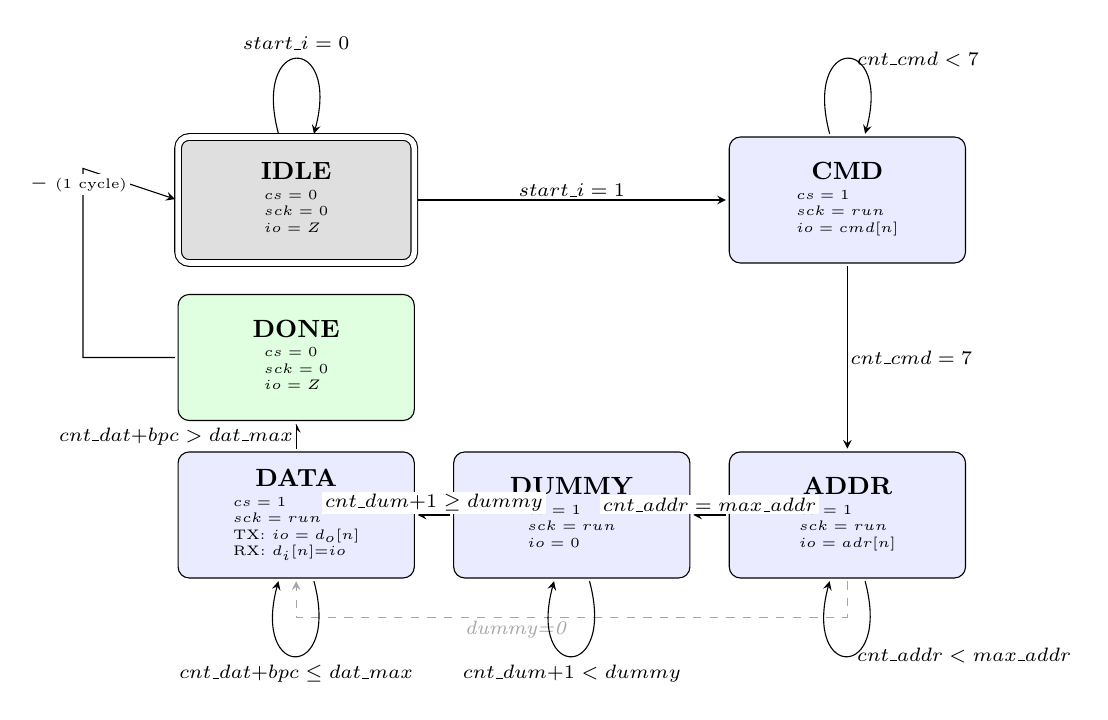
\begin{tikzpicture}[
    >=stealth,
    shorten >=1pt, shorten <=1pt,
    state/.style={
      draw, rounded corners=4pt,
      minimum width=3.0cm, minimum height=1.6cm,
      align=center, font=\small
    },
    reset/.style={state, fill=gray!25, double, double distance=2pt},
    active/.style={state, fill=blue!8},
    done/.style={state, fill=green!12},
    lbl/.style={font=\scriptsize, fill=white, inner sep=1pt, midway},
    lbll/.style={font=\scriptsize, fill=white, inner sep=1pt, midway, left},
    lblr/.style={font=\scriptsize, fill=white, inner sep=1pt, midway, right},
    lbla/.style={font=\scriptsize, fill=white, inner sep=1pt, midway, above},
    lblb/.style={font=\scriptsize, fill=white, inner sep=1pt, midway, below},
  ]

  % ── Nodes ──────────────────────────────────────────────────
  %  IDLE   (0 , 6)
  %  CMD    (7 , 6)
  %  ADDR   (7 , 2)
  %  DUMMY  (3.5, 2)
  %  DATA   (0 , 2)
  %  DONE   (0 , 4)

  \node[reset] (IDLE) at (0,6) {
    \textbf{IDLE}\\[2pt]
    \tiny\begin{tabular}{l}
      $cs=0$\\ $sck=0$\\ $io=Z$
    \end{tabular}
  };

  \node[active] (CMD) at (7,6) {
    \textbf{CMD}\\[2pt]
    \tiny\begin{tabular}{l}
      $cs=1$\\ $sck=\text{run}$\\ $io=cmd[n]$
    \end{tabular}
  };

  \node[active] (ADDR) at (7,2) {
    \textbf{ADDR}\\[2pt]
    \tiny\begin{tabular}{l}
      $cs=1$\\ $sck=\text{run}$\\ $io=adr[n]$
    \end{tabular}
  };

  \node[active] (DUMMY) at (3.5,2) {
    \textbf{DUMMY}\\[2pt]
    \tiny\begin{tabular}{l}
      $cs=1$\\ $sck=\text{run}$\\ $io=0$
    \end{tabular}
  };

  \node[active] (DATA) at (0,2) {
    \textbf{DATA}\\[2pt]
    \tiny\begin{tabular}{l}
      $cs=1$\\ $sck=\text{run}$\\
      TX: $io=d_{o}[n]$\\
      RX: $d_{i}[n]{=}io$
    \end{tabular}
  };

  \node[done] (DONE) at (0,4) {
    \textbf{DONE}\\[2pt]
    \tiny\begin{tabular}{l}
      $cs=0$\\ $sck=0$\\ $io=Z$
    \end{tabular}
  };

  % ── Transitions ─────────────────────────────────────────────

  % IDLE self-loop
  \draw[->] (IDLE) edge[loop above]
    node[above, font=\scriptsize] {$start\_i=0$}
    (IDLE);

  % IDLE → CMD
  \draw[->] (IDLE) -- (CMD)
    node[lbla] {$start\_i=1$};

  % CMD self-loop
  \draw[->] (CMD) edge[loop above]
    node[right, font=\scriptsize] {$cnt\_cmd < 7$}
    (CMD);

  % CMD → ADDR
  \draw[->] (CMD) -- (ADDR)
    node[lblr] {$cnt\_cmd = 7$};

  % ADDR self-loop
  \draw[->] (ADDR) edge[loop below]
    node[right, font=\scriptsize] {$cnt\_addr < max\_addr$}
    (ADDR);

  % ADDR → DUMMY  (normal path)
  \draw[->] (ADDR) -- (DUMMY)
    node[lbla] {$cnt\_addr = max\_addr$};

  % ADDR → DATA  (shortcut: dummy_reg_i = 0, dashed)
  \draw[->, dashed, gray!70]
    (ADDR.south) -- ++(0,-0.5) -| (DATA.south)
    node[lblb, pos=0.3] {\textit{dummy=0}};

  % DUMMY self-loop
  \draw[->] (DUMMY) edge[loop below]
    node[below, font=\scriptsize] {$cnt\_dum{+}1 < dummy$}
    (DUMMY);

  % DUMMY → DATA
  \draw[->] (DUMMY) -- (DATA)
    node[lbla] {$cnt\_dum{+}1 \geq dummy$};

  % DATA self-loop
  \draw[->] (DATA) edge[loop below]
    node[below, font=\scriptsize] {$cnt\_dat{+}bpc \leq dat\_max$}
    (DATA);

  % DATA → DONE
  \draw[->] (DATA) -- (DONE)
    node[lbll] {$cnt\_dat{+}bpc > dat\_max$};

  % DONE → IDLE  (links außen, klar sichtbar)
  \draw[->] (DONE.west) -- ++(-1.2,0) -- ++(0,2.4) -- (IDLE.west)
    node[lbll, pos=0.5] {$-$ \tiny(1 cycle)};

\end{tikzpicture}
\caption{QSPI Kernel Moore-FSM. Doppelter Rahmen = Reset-Zustand IDLE (grau).
  Grüner Rahmen = DONE (1 Zyklus, bedingungslos zu IDLE).
  Gestrichelter Pfad: ADDR\,$\to$\,DATA wenn \texttt{DUMMY\_CYC}\,$=$\,0.}
\label{fig:asqspi02}
\end{figure}







Table \ref{tab:asqspi_cnt} shows the kernel internel counters for the different parts of the SPI waveform.
\begin{table}[H]
\caption{\texttt{as\_qspi} Internal Counters}
\label{tab:asqspi_cnt}
\centering
\begin{tabularx}{\textwidth}{|l|l|X|}
  \hline
  Counter & Width & Description \\
  \hline\hline
  \texttt{sck\_cnt\_r}  & 8 & SCK clock divider counter. Resets to \texttt{clkdiv\_reg\_i}. \\
  \hline
  \texttt{cnt\_cmd\_r}  & 3 & CMD phase bit counter. Counts 0..7 (always 8 bits, single wire). \\
  \hline
  \texttt{cnt\_addr\_r} & 5 & ADDR phase bit counter. Max = 23 (3-byte) or 31 (4-byte). \\
  \hline
  \texttt{cnt\_dum\_r}  & 6 & DUMMY cycle counter. Counts up to \texttt{dummy\_reg\_i}. \\
  \hline
  \texttt{cnt\_dat\_r}  & 20 & DAT phase bit counter. Counts in steps of \texttt{bpc\_s}. Max = \texttt{len\_reg\_i*8 - 1}. \\
  \hline
\end{tabularx}
\end{table}

%%%%%%%%%%%%%%%%%%%%%%%%%%%%%%%%%
% Functional Overview: Timing Constraints
%%%%%%%%%%%%%%%%%%%%%%%%%%%%%%%%%
\subsubsection{Timing Constraints}

\begin{itemize}
  \item All configuration registers (\texttt{cmd\_reg\_i}, \texttt{addr\_reg\_i},
    \texttt{len\_reg\_i}, etc.) must be stable before \texttt{start\_i} is asserted
    and must remain stable for the duration of the transfer (BUSY=1).
  \item \texttt{clkdiv\_reg\_i} must not change while BUSY=1.
  \item \texttt{tx\_data\_i} must be valid when \texttt{tx\_rd\_o} fires. The BPI
    preloads the TX shift register one cycle before DAT\_ST.
  \item \texttt{rx\_data\_o} is valid two clock cycles after \texttt{rx\_wr\_o}
    (NBA settling time in simulation; in synthesis: same cycle is valid).
\end{itemize}

%%%%%%%%%%%%%%%%%%%%%%%%%%%%%%%%%
% Functional Overview: Functional Description QSPI-BPI
%%%%%%%%%%%%%%%%%%%%%%%%%%%%%%%%%
\subsubsection{Functional Description QSPI-BPI}

The \texttt{as\_slave\_bpi} module implements a Wishbone Classic Compliant Slave
BPI. It provides zero-wait-state single read/write transfers to the attached
peripheral (QSPI top level). The BPI is fully combinatorial on the bus side;
ACK is asserted in the same clock cycle as STB.

\paragraph{Protocol:}
A valid Wishbone transfer requires \texttt{CYC\_I = 1} and \texttt{STB\_I = 1}
simultaneously. All SEL bits must be asserted (\texttt{SEL\_I = 0xFF}) for a
transfer to be acknowledged. The ACK is combinatorial:
\[
  ACK\_O = CYC\_I \;\land\; STB\_I \;\land\; (\&SEL\_I)
\]

\paragraph{Write:}
When \texttt{WE\_I = 1}, \texttt{WR\_O} is asserted to the peripheral for the
duration of the bus cycle. The address decoder in the Top level routes the write
to the appropriate register.

\paragraph{Read:}
When \texttt{WE\_I = 0}, \texttt{RD\_O} is asserted. The peripheral must provide
read data combinatorially on \texttt{DAT\_FROM\_CORE\_I}; this is passed
directly to \texttt{WB\_S\_DAT\_O}.

%%%%%%%%%%%%%%%%%%%%%%%%%%%%%%%%%
% Functional Overview: Functional Description QSPI-Top-Level
%%%%%%%%%%%%%%%%%%%%%%%%%%%%%%%%%
\subsubsection{Functional Description QSPI-Top-Level}

\texttt{as\_qspi\_top} integrates the Wishbone BPI (\texttt{as\_slave\_bpi}),
the QSPI kernel (\texttt{as\_qspi}), the TX FIFO, and the RX FIFO into a
complete memory-mapped QSPI peripheral. It decodes the register offset address,
routes read/write strobes to the appropriate registers, and implements the
interrupt logic.

\paragraph{Register Address Decoding:}
The BPI passes the raw bus address directly as a byte offset. The Top level
compares this offset against the constants defined in Table~\ref{tab:asqspitop_regmap}
using combinatorial equality. There is no base-address stripping; the bus master
must provide the byte offset from the peripheral's base address.

\paragraph{Start Pulse Generation:}
Writing \texttt{CTRL.START (bit 3) = 1} causes the Top level to register the
write strobe for one clock cycle:
\[
  start\_r \;\leftarrow\; wr\_ctrl \;\land\; data\_wr\_s[3]
\]
\[
  start\_s = start\_r \quad \text{(one-cycle pulse, registered)}
\]

\paragraph{FIFO Flush:}
\texttt{CTRL.TX\_FLUSH (bit 1)} and \texttt{CTRL.RX\_FLUSH (bit 2)} are
combinatorial and active only during the write cycle:
\[
  tx\_flush\_s = wr\_ctrl \;\land\; data\_wr\_s[1]
\]
\[
  rx\_flush\_s = wr\_ctrl \;\land\; data\_wr\_s[2]
\]
Flushing while BUSY is asserted is implementation-defined; in this
implementation the flush takes effect immediately.

\paragraph{RX FIFO Write Pipeline:}
The kernel outputs \texttt{rx\_wr\_o} and \texttt{rx\_data\_o} (\texttt{rx\_shift\_r})
as NBA assignments in the same clock cycle. To avoid a simulation race condition
(and to provide a registered interface for synthesis), a two-cycle pipeline
is used:
\begin{itemize}
  \item Cycle N: \texttt{rx\_wr\_kernel\_s = 1}, \texttt{rx\_shift\_r} NBA pending.
  \item Cycle N+1: \texttt{rx\_wr\_d1 = 1}, \texttt{rx\_data\_kernel\_s} captured
    into \texttt{rx\_data\_snap} (shift register now settled).
  \item Cycle N+2: \texttt{rx\_wr\_d2 = 1}, \texttt{rx\_data\_snap} written to RX FIFO.
\end{itemize}

\paragraph{RX FIFO Pop (read-before-pop):}
Reading \texttt{RXDATA} presents \texttt{mem[rd\_ptr\_r]} combinatorially and
schedules the pointer advance one cycle later via \texttt{rx\_pop\_r}. This
separates data presentation from pointer advancement and is required for
correct operation with the asynchronous-read \texttt{as\_fifo}.


%%%%%%%%%%%%%%%%%%%%%%%%%%%%%%%%%
% Structural Overview
%%%%%%%%%%%%%%%%%%%%%%%%%%%%%%%%%
\subsection{Structural Overview}
The QSPI controller is a dual-port peripheral: it is accessed from the Wishbone bus for
configuration (register file, FIFOs, interrupts) and from the AXI4 bus for cache-refill
data transfers. Both clock domains are synchronous to \texttt{clk\_i}. Figure \ref{fig:asqspi01}
shows the block diagram.

\begin{figure}[H]
\centering
\begin{tikzpicture}[>=stealth]
% ── background bands ──────────────────────────────────────────
\filldraw[fill=lightgray!60, draw=black] (0,0) rectangle (12,4);
\filldraw[fill=lightgray!30, draw=black] (0,4) rectangle (12,7);
% ── kernel block ──────────────────────────────────────────────
\filldraw[fill=white, draw=black] (2,5) rectangle (10,6);
\node at (6,5.5) {QSPI peripheral kernel};
% ── bus-domain sub-blocks ─────────────────────────────────────
\draw (1.5,4) node[draw,fill=white,align=center] {Clock Gating \\ Block};
\draw (4.0,4) node[draw,fill=white,align=center] {Sync. \\ Block};
\draw (2.0,2.5) node[draw,fill=white,align=center] {Service Request \\ Block};
\draw (5.5,2.5) node[draw,fill=white,align=center] {SFR \\ Block};
\draw (8.0,2.5) node[draw,fill=white,align=center] {TX \\ FIFO};
\draw (9.5,2.5) node[draw,fill=white,align=center] {RX \\ FIFO};
% ── BPI blocks ────────────────────────────────────────────────
\draw (3.5,0.4) node[draw,fill=blue!10,text=blue!70!black] {WB Slave BPI};
\draw (8.5,0.4) node[draw,fill=red!10, text=red!70!black]  {AXI4 Slave BPI};
% ── domain labels ─────────────────────────────────────────────
\node[font=\small] at (10.2,4.25) {Kernel clock domain};
\node[font=\small] at (10.2,0.25) {Bus clock domain};
% ── NOR-Flash (top) ───────────────────────────────────────────
\draw (6,9.2) node[draw,fill=white] {NOR-Flash};
\draw[<->] (6,7) -- (6,8.9) node[midway,sloped,above=2pt,font=\small] {\asqspiData\;[3:0]};
\draw[->]  (5,7) -- (5,8.9) node[midway,sloped,above=2pt,font=\small] {\asqspiSCK};
\draw[->]  (7,7) -- (7,8.9) node[midway,sloped,above=2pt,font=\small] {\asqspiCS};
% ── IRQ ───────────────────────────────────────────────────────
\draw[->] (1,-0.2) -- (1,-0.9);
\node[left,font=\small] at (1,-0.6) {qspi\_irq\_o};
% ── Wishbone bus (blue, left) ─────────────────────────────────
\node[double arrow,draw,fill=blue!10,text=blue!70!black,
      minimum height=0.8cm,font=\small] at (3.5,-1.8) {Wishbone B4};
\draw[blue!70!black,->] (3.5,-1.3) -- (3.5,-0.8);
% ── AXI4 bus (red, right) ─────────────────────────────────────
\node[double arrow,draw,fill=red!10,text=red!70!black,
      minimum height=0.8cm,font=\small] at (8.5,-1.8) {AXI4 (AR+R)};
\draw[red!70!black,->] (8.5,-1.3) -- (8.5,-0.8);
\end{tikzpicture}
\caption{QSPI Dual-Port Peripheral (Wishbone config + AXI4 data)}
\label{fig:asqspi01}
\end{figure}

\paragraph{QSPI Peripheral Kernel: } The QSPI kernel provides the specific functionality of the QSPI interface, described in Section \ref{subsec:qspifunc02}. It runs in the system clock domain.

\paragraph{Wishbone Slave BPI: } Connects the QSPI configuration registers to the system Wishbone bus. Zero-wait-state, 64-bit. Handles all SW register accesses, FIFO reads/writes, and interrupt register updates.

\paragraph{AXI4 Slave BPI: } Accepts cache-refill read requests from the Memory Arbiter via the AXI4 read channels (AR+R). Executes a Quad Fast Read (opcode 0x6B) on the NOR-Flash for each ARLEN=3 burst and returns 4~$\times$~64-bit beats (32~bytes = one cache line) with \texttt{RLAST} asserted on the fourth beat.

\paragraph{asSlaveBPI Block: } The Wishbone BPI block lies within the bus clock domain and contains the following subblocks:
\begin{description}
  \item [Special Function Register Block] The Special Function Register Block contains all FIFO specific registers and all special function registers (SFR) of the peripheral kernel that are accessible by the SW via the system bus.
  \item [Service Request Block SRB] The SRB is used to prepare the interrupt and data transfer requests for the Interrupt Control Unit (ICU) and the DMA Controller (DMAC), respectively (no DMA planned!).
  \item [TX FIFO] The TX FIFO is used to buffer the transmission data from the bus, in order to adapt the character processing speed of the peripheral kernel to the transfer rate of the system bus.
  \item [RX FIFO] The RX FIFO is used to buffer the received data from the kernel, in order to adapt the character processing speed of the peripheral kernel to the transfer rate of the bus system.
\end{description}

\paragraph{Clock Gating Block: } The Clock Gating Block is used to derive the necessary clocks for the several blocks within the peripheral from the clocks provided by the system.

\paragraph{Synchronization Block: } The Synchronization Block is used to synchronize the signals between the bus clock and kernel clock domains.

%%%%%%%%%%%%%%%%%%%%%%%%%%%%%%%%%
% Structural Overview: I/O of the QSPI Kernel
%%%%%%%%%%%%%%%%%%%%%%%%%%%%%%%%%
\subsubsection{I/O of the QSPI Kernel}

Table \ref{tab:asQspiPer04a}, \ref{tab:asQspiPer04ab}  shows the input and outputs of the QSPI kernel.

\begin{table}[H]
\caption{\texttt{as\_qspi} Ports -- System and Configuration}
\label{tab:asQspiPer04a}
\centering
\begin{tabularx}{\textwidth}{|l|l|l|X|}
  \hline
  Port & Dir. & Width & Description \\
  \hline\hline
  \texttt{clk\_i}           & in  & 1  & Kernel clock, active rising edge \\
  \hline
  \texttt{rst\_i}           & in  & 1  & Synchronous reset, active high \\
  \hline
  \texttt{start\_i}         & in  & 1  & Start pulse (one cycle wide). Initiates FSM if not busy. \\
  \hline
  \texttt{ctrl\_reg\_i}     & in  & 8  & Packed \texttt{qspi\_ctrl\_t}: \{addr\_len, cpol, cpha, dual, cs\_hold, xip, ddr, quad\} \\
  \hline
  \texttt{cmd\_reg\_i}      & in  & 8  & SPI opcode byte \\
  \hline
  \texttt{addr\_reg\_i}     & in  & 32 & Flash target address \\
  \hline
  \texttt{len\_reg\_i}      & in  & 16 & Transfer length in bytes \\
  \hline
  \texttt{dummy\_reg\_i}    & in  & 6  & Number of dummy cycles \\
  \hline
  \texttt{clkdiv\_reg\_i}   & in  & 8  & SCK clock divider \\
  \hline
  \texttt{timeout\_reg\_i}  & in  & 32 & Timeout threshold in clock cycles; 0 = disabled \\
  \hline
  \texttt{xip\_mode\_bits\_i}& in & 8  & XIP mode byte, driven on IO[3:0] during XIP address phase \\
  \hline
\end{tabularx}
\end{table}

\begin{table}[H]
\caption{\texttt{as\_qspi} Ports -- Status, FIFO and SPI}
\label{tab:asQspiPer04ab}
\centering
\begin{tabularx}{\textwidth}{|l|l|l|X|}
  \hline
  Port & Dir. & Width & Description \\
  \hline\hline
  \texttt{stat\_busy\_o}    & out & 1  & FSM is active (not IDLE, not DONE). Level signal. \\
  \hline
  \texttt{stat\_done\_o}    & out & 1  & FSM is in DONE state. High for exactly one clock cycle. \\
  \hline
  \texttt{stat\_error\_o}   & out & 1  & Error latched. Remains until ICR clear. \\
  \hline
  \texttt{stat\_timeout\_o} & out & 1  & Timeout occurred. Remains until ICR clear. \\
  \hline
  \texttt{xip\_active\_o}   & out & 1  & XIP mode is active. \\
  \hline
  \texttt{tx\_empty\_i}     & in  & 1  & TX FIFO empty indication (from TX FIFO or BPI) \\
  \hline
  \texttt{tx\_rd\_o}        & out & 1  & TX FIFO read strobe. One cycle pulse on last TX drive. \\
  \hline
  \texttt{tx\_data\_i}      & in  & 64 & TX data word from TX FIFO \\
  \hline
  \texttt{rx\_full\_i}      & in  & 1  & RX FIFO full indication \\
  \hline
  \texttt{rx\_wr\_o}        & out & 1  & RX FIFO write strobe. One cycle pulse on last RX sample. \\
  \hline
  \texttt{rx\_data\_o}      & out & 64 & RX shift register output. Valid after \texttt{rx\_wr\_o}. \\
  \hline
  \texttt{sck\_o}           & out & 1  & SPI clock output \\
  \hline
  \texttt{cs\_o}            & out & 1  & Chip select (active high). Deasserted in IDLE and DONE. \\
  \hline
  \texttt{data\_io}         & inout & 4 & SPI data bus (tri-state). Driven in CMD/ADDR/TX-DAT, sampled in RX-DAT. \\
  \hline
\end{tabularx}
\end{table}

%%%%%%%%%%%%%%%%%%%%%%%%%%%%%%%%%
% Structural Overview: I/O of the QSPI BPI
%%%%%%%%%%%%%%%%%%%%%%%%%%%%%%%%%
\subsubsection{I/O of the QSPI BPI}
Table \ref{tab:asQspiPer05} shows the input and outputs of the QSPI BPI.

\begin{table}[H]
\caption{\texttt{as\_slave\_bpi} Ports}
\label{tab:asQspiPer05}
\centering
\begin{tabularx}{\textwidth}{|l|l|l|X|}
  \hline
  Port & Dir. & Width & Description \\
  \hline\hline
  \texttt{rst\_i}             & in  & 1  & System reset, active high (unused internally; for consistency) \\
  \hline
  \texttt{clk\_i}             & in  & 1  & System clock (unused internally; for consistency) \\
  \hline
  \multicolumn{4}{|l|}{\textit{Peripheral (kernel) side:}} \\
  \hline
  \texttt{addr\_o}            & out & 64 & Decoded byte offset address, directly from \texttt{wb\_s\_addr\_i} \\
  \hline
  \texttt{dat\_from\_core\_i} & in  & 64 & Read data from peripheral, presented combinatorially \\
  \hline
  \texttt{dat\_to\_core\_o}   & out & 64 & Write data to peripheral, directly from \texttt{wb\_s\_dat\_i} \\
  \hline
  \texttt{wr\_o}              & out & 1  & Write enable to peripheral. Combinatorial. \\
  \hline
  \texttt{rd\_o}              & out & 1  & Read enable to peripheral. Combinatorial. \\
  \hline
  \multicolumn{4}{|l|}{\textit{Wishbone slave side:}} \\
  \hline
  \texttt{wb\_s\_addr\_i}     & in  & 64 & Wishbone address (byte offset from peripheral base) \\
  \hline
  \texttt{wb\_s\_dat\_i}      & in  & 64 & Wishbone write data \\
  \hline
  \texttt{wb\_s\_dat\_o}      & out & 64 & Wishbone read data \\
  \hline
  \texttt{wb\_s\_we\_i}       & in  & 1  & Wishbone write enable \\
  \hline
  \texttt{wb\_s\_sel\_i}      & in  & 8  & Wishbone byte select (all bytes must be selected) \\
  \hline
  \texttt{wb\_s\_stb\_i}      & in  & 1  & Wishbone strobe (valid cycle) \\
  \hline
  \texttt{wb\_s\_ack\_o}      & out & 1  & Wishbone acknowledge (combinatorial, zero wait state) \\
  \hline
  \texttt{wb\_s\_cyc\_i}      & in  & 1  & Wishbone cycle (high for complete bus transaction) \\
  \hline
\end{tabularx}
\end{table}

%%%%%%%%%%%%%%%%%%%%%%%%%%%%%%%%%
% Structural Overview: Internals of the QSPI BPI
%%%%%%%%%%%%%%%%%%%%%%%%%%%%%%%%%
\subsubsection{Internals of the QSPI BPI}
Table \ref{tab:asQspiPer07} shows the internal signals and processes of the QSPI BPI.
\begin{table}[H]
\caption{QSPI BPI Internals}
\label{tab:asQspiPer07}
\centering
\begin{tabularx}{\textwidth}{|l |l |l |X|}
  \hline
  Object & Type & Width & Explanation \\
  \hline
  \hline
  any & logic & x & See BPI spec. \\
  \hline
\end{tabularx}
\end{table}

%%%%%%%%%%%%%%%%%%%%%%%%%%%%%%%%%
% Structural Overview: BPI Transfer Timing
%%%%%%%%%%%%%%%%%%%%%%%%%%%%%%%%%
\subsubsection{BPI Transfer Timing}

\begin{table}[H]
\caption{Wishbone Classic Zero-Wait-State Timing}
\label{tab:asbpi_timing}
\centering
\begin{tabularx}{\textwidth}{|l|X|}
  \hline
  Cycle & Description \\
  \hline\hline
  T0 & Master asserts CYC, STB, ADR, DAT (write) or ADR (read), WE, SEL \\
  \hline
  T0 & Slave combinatorially asserts ACK. Read data appears on DAT\_O. \\
  \hline
  T1 & Master samples ACK and DAT\_O on rising clock edge. \\
  \hline
  T1 & Master deasserts STB (and CYC for single transfers). \\
  \hline
\end{tabularx}
\end{table}

\textbf{Note:} The peripheral register file is clocked (\texttt{always\_ff}),
so a write takes effect on the posedge of the clock during which \texttt{WR\_O}
is asserted. Read data must be available combinatorially before the posedge.

%%%%%%%%%%%%%%%%%%%%%%%%%%%%%%%%%
% Structural Overview: I/O of the QSPI AXI4 Slave Port
%%%%%%%%%%%%%%%%%%%%%%%%%%%%%%%%%
\subsubsection{I/O of the QSPI AXI4 Slave Port}
\label{subsec:qspiAxi4Port}

Table~\ref{tab:asQspiAxi4} lists the AXI4 slave signals of the QSPI data port.
Only the read channels (AR and R) are implemented; write channels (AW, W, B) are absent.
All signals are synchronous to \texttt{clk\_i}.

\begin{table}[H]
\caption{\texttt{as\_qspi\_top} AXI4 Slave Port Signals (AR + R channels only)}
\label{tab:asQspiAxi4}
\centering
\begin{tabularx}{\textwidth}{|l|l|l|X|}
  \hline
  Signal & Dir. & Width & Description \\
  \hline\hline
  \multicolumn{4}{|l|}{\textit{AR channel (Address Read):}} \\
  \hline
  \texttt{axi\_s\_arvalid\_i} & in  & 1  & Master presents a valid read-address transaction \\
  \hline
  \texttt{axi\_s\_arready\_o} & out & 1  & Slave ready to accept address. Asserted when not busy. \\
  \hline
  \texttt{axi\_s\_arid\_i}    & in  & 4  & Transaction ID. Echoed back on R channel. \\
  \hline
  \texttt{axi\_s\_araddr\_i}  & in  & 32 & Byte address of first beat (must be 32-byte aligned) \\
  \hline
  \texttt{axi\_s\_arlen\_i}   & in  & 4  & Burst length minus 1 (always 3; 4 beats per transaction) \\
  \hline
  \texttt{axi\_s\_arsize\_i}  & in  & 3  & Beat size code (always 3 = 8~bytes = 64~bit) \\
  \hline
  \texttt{axi\_s\_arburst\_i} & in  & 2  & Burst type (always INCR = 2'b01) \\
  \hline
  \multicolumn{4}{|l|}{\textit{R channel (Read Data):}} \\
  \hline
  \texttt{axi\_s\_rvalid\_o}  & out & 1  & Slave presents valid read data \\
  \hline
  \texttt{axi\_s\_rready\_i}  & in  & 1  & Master ready to accept data \\
  \hline
  \texttt{axi\_s\_rid\_o}     & out & 4  & Transaction ID (echo of \texttt{axi\_s\_arid\_i}) \\
  \hline
  \texttt{axi\_s\_rdata\_o}   & out & 64 & Read data (one beat = 8~bytes of flash data) \\
  \hline
  \texttt{axi\_s\_rresp\_o}   & out & 2  & Response: OKAY (2'b00) or SLVERR (2'b10) on flash error \\
  \hline
  \texttt{axi\_s\_rlast\_o}   & out & 1  & Asserted on the 4th and final beat of each burst \\
  \hline
\end{tabularx}
\end{table}

\paragraph{Transaction Sequence:}
\begin{enumerate}
  \item Master (Memory Arbiter) asserts \texttt{ARVALID} with address, ID, ARLEN=3, ARSIZE=3, ARBURST=INCR.
  \item Slave asserts \texttt{ARREADY} when idle; address is latched on the handshake cycle.
  \item Slave initiates a Quad Fast Read (opcode 0x6B) on the NOR-Flash.
  \item Slave returns 4 data beats on the R channel, asserting \texttt{RVALID} per beat and \texttt{RLAST} on beat~4.
  \item On a flash error (timeout or kernel error), \texttt{RRESP} = SLVERR on the affected beat; the cache controller maps this to a RISC-V access-fault exception (mcause = 1 for I-Cache, 5 for D-Cache).
\end{enumerate}

%%%%%%%%%%%%%%%%%%%%%%%%%%%%%%%%%
% Structural Overview: I/O of the QSPI Top
%%%%%%%%%%%%%%%%%%%%%%%%%%%%%%%%%
\subsubsection{I/O of the QSPI Top}

Table \ref{tab:asQspiPer06} shows the input and outputs of the QSPI Top.

\begin{table}[H]
\caption{\texttt{as\_qspi\_top} Ports -- System, Wishbone, and SPI}
\label{tab:asQspiPer06}
\centering
\begin{tabularx}{\textwidth}{|l|l|l|X|}
  \hline
  Port & Dir. & Width & Description \\
  \hline\hline
  \texttt{rst\_i}       & in  & 1  & Synchronous reset, active high \\
  \hline
  \texttt{clk\_i}       & in  & 1  & System and kernel clock \\
  \hline
  \multicolumn{4}{|l|}{\textit{Wishbone slave port (configuration):}} \\
  \hline
  \texttt{wbdAddr\_i}   & in  & 64 & Wishbone address (byte offset from QSPI base) \\
  \hline
  \texttt{wbdDat\_i}    & in  & 64 & Wishbone write data \\
  \hline
  \texttt{wbdDat\_o}    & out & 64 & Wishbone read data \\
  \hline
  \texttt{wbdWe\_i}     & in  & 1  & Wishbone write enable \\
  \hline
  \texttt{wbdSel\_i}    & in  & 8  & Wishbone byte select \\
  \hline
  \texttt{wbdStb\_i}    & in  & 1  & Wishbone strobe \\
  \hline
  \texttt{wbdAck\_o}    & out & 1  & Wishbone acknowledge \\
  \hline
  \texttt{wbdCyc\_i}    & in  & 1  & Wishbone cycle \\
  \hline
  \multicolumn{4}{|l|}{\textit{AXI4 slave port (cache-refill data, AR+R channels only):}} \\
  \hline
  \texttt{axi\_s\_arvalid\_i} & in  & 1  & AR valid \\
  \hline
  \texttt{axi\_s\_arready\_o} & out & 1  & AR ready \\
  \hline
  \texttt{axi\_s\_arid\_i}    & in  & 4  & AR transaction ID \\
  \hline
  \texttt{axi\_s\_araddr\_i}  & in  & 32 & AR byte address (32-byte aligned) \\
  \hline
  \texttt{axi\_s\_arlen\_i}   & in  & 4  & AR burst length (fixed 3 = 4 beats) \\
  \hline
  \texttt{axi\_s\_arsize\_i}  & in  & 3  & AR beat size (fixed 3 = 8\,bytes) \\
  \hline
  \texttt{axi\_s\_arburst\_i} & in  & 2  & AR burst type (fixed INCR = 2'b01) \\
  \hline
  \texttt{axi\_s\_rvalid\_o}  & out & 1  & R valid \\
  \hline
  \texttt{axi\_s\_rready\_i}  & in  & 1  & R ready \\
  \hline
  \texttt{axi\_s\_rid\_o}     & out & 4  & R transaction ID (echo of arid) \\
  \hline
  \texttt{axi\_s\_rdata\_o}   & out & 64 & R data \\
  \hline
  \texttt{axi\_s\_rresp\_o}   & out & 2  & R response (OKAY / SLVERR) \\
  \hline
  \texttt{axi\_s\_rlast\_o}   & out & 1  & R last beat \\
  \hline
  \multicolumn{4}{|l|}{\textit{SPI / Flash and interrupt:}} \\
  \hline
  \texttt{sck\_o}       & out & 1  & SPI clock to NOR-Flash \\
  \hline
  \texttt{cs\_o}        & out & 1  & Chip select to NOR-Flash (active high) \\
  \hline
  \texttt{data\_io}     & inout & 4 & QSPI data bus to/from NOR-Flash \\
  \hline
  \texttt{qspi\_irq\_o} & out & 1  & Interrupt request to CPU interrupt controller \\
  \hline
\end{tabularx}
\end{table}

Table \ref{tab:asQspiPer06a} shows the internals  of the QSPI Top.
\begin{table}[H]
\caption{QSPI Top Signals}
\label{tab:asQspiPer06a}
\centering
\begin{tabularx}{\textwidth}{|l |l |X|}
  \hline
  Signal & Width & Explanation \\
  \hline
  \hline
  tbd  & 1 & tbd \\
  \hline
\end{tabularx}
\end{table}

%%%%%%%%%%%%%%%%%%%%%%%%%%%%%%%%%
% Service Requests of the QSPI
%%%%%%%%%%%%%%%%%%%%%%%%%%%%%%%%%
\subsection{Service Requests of the QSPI}
Interrupt sources are level-based and derived directly from kernel status
or FIFO fill levels.

The details will be shown in section \ref{subsub:IRQRegs}.


%%%%%%%%%%%%%%%%%%%%%%%%%%%%%%%%%
% The QSPI Peripheral Kernel
%%%%%%%%%%%%%%%%%%%%%%%%%%%%%%%%%
\subsection{The QSPI Peripheral Kernel}
\label{subsec:qspifunc02}
\paragraph{Block Architecture} -:
The block architecture is like:
\begin{verbatim}
Wishbone (config)      AXI4 AR+R (data / cache-refill)
       |                          |
  WB Slave BPI             AXI4 Slave BPI
       |                          |
Register File + IRQ Logic (SRB)   |
       \__________________________|
                    |
             QSPI Kernel FSM
                    |
          TX FIFO / RX FIFO
                    |
       SPI PHY (SCK / CS / IO[3:0])
\end{verbatim}

The kernel is fully state-driven and does not depend on external events such as interrupts or bus timing.

Writing bit 3 of \asqspiCtrlRegExt\textbf{.START} initiates a transaction if not busy.

\paragraph{Design Rules} -:
\begin{itemize}
  \item The kernel FSM is fully state-driven.
  \item No FSM state depends on interrupt signals.
  \item Interrupts never control hardware behavior.
  \item All external behavior is driven by register state only.
\end{itemize}

%%%%%%%%%%%%%%%%%%%%%%%%%%%%%%%%%%%%%%%%%%
% All Registers
%%%%%%%%%%%%%%%%%%%%%%%%%%%%%%%%%%%%%%%%%%
\subsection{Registers}
In the following the registers of a QSPI peripheral are listed and described. Some registers’ layout or availability depends on the generic feature set implemented for that QSPI’s instantiation. Such registers and concerned bit fields are denoted by the use of italic style.

%%%%%%%%%%%%%%%%%%%%%%%%%%%%%%%%%%%%%%%%%%
% All Registers: Register Overview
%%%%%%%%%%%%%%%%%%%%%%%%%%%%%%%%%%%%%%%%%%
\subsubsection{QSPI Register Overview}

\begin{table}[H]
\caption{\texttt{as\_qspi\_top} Register Map}
\label{tab:asqspitop_regmap}
\centering
\begin{tabularx}{\textwidth}{|l|l| X| l| X|}
  \hline
  Offset & Symbol & Reset & Access & Description \\
  \hline\hline
  0x00 (0)   & ID        & \footnotesize{0x00000000\_00000010} & r   & Peripheral identification register \\
  \hline
  0x08 (8)   & CTRL      & \footnotesize{0x00000000\_00000000} & rw  & Control register (START, FLUSH, mode bits) \\
  \hline
  0x10 (16)  & CMD       & \footnotesize{0x00000000\_00000000} & rw  & SPI opcode \\
  \hline
  0x18 (24)  & ADDR      & \footnotesize{0x00000000\_00000000} & rw  & Flash target address \\
  \hline
  0x20 (32)  & LEN       & \footnotesize{0x00000000\_00000000} & rw  & Transfer length in bytes \\
  \hline
  0x28 (40)  & DUMMY   &  \footnotesize{0x00000000\_00000000} & rw  & Dummy cycles \\
  \hline
  0x30 (48)  & CLKDIV    & \footnotesize{0x00000000\_00000000} & rw  & SCK clock divider \\
  \hline
  0x38 (56)  & TIMEOUT   & \footnotesize{0x00000000\_00000000} & rw  & Timeout threshold \\
  \hline
  0x40 (64)  & ISR       & \footnotesize{0x00000000\_00000000} & w   & Interrupt Set Register (w1 $\to$ set RIS) \\
  \hline
  0x48 (72)  & RIS       & \footnotesize{0x00000000\_00000000} & rh  & Raw Interrupt Status Register \\
  \hline
  0x50 (80)  & IMSC      & \footnotesize{0xFFFFFFFF\_FFFFFFFF} & rw  & Interrupt Mask Control Register \\
  \hline
  0x58 (88)  & MIS       & \footnotesize{0x00000000\_00000000} & rh  & Masked Interrupt Status (= RIS \& IMSC) \\
  \hline
  0x60 (96)  & ICR       & \footnotesize{0x00000000\_00000000} & w   & Interrupt Clear Register (w1 $\to$ clear RIS) \\
  \hline
  0x68 (104) & RXDATA    & \footnotesize{0x00000000\_00000000} & r   & RX FIFO pop (read-before-pop) \\
  \hline
  0x70 (112) & TXDATA    & \footnotesize{0x00000000\_00000000} & w   & TX FIFO push \\
  \hline
  0x78 (120) & FIFOSTAT  & \footnotesize{0x00000000\_00000000} & rh  & FIFO fill levels and flags \\
  \hline
  0x80 (128) & XIPMODE   & \footnotesize{0x00000000\_000000A0} & rw  & XIP mode byte (Winbond default: 0xA0) \\
  \hline
  0x88 (136) & STATUS    & \footnotesize{0x00000000\_00000000} & rh  & Kernel status flags \\
  \hline
\end{tabularx}
\end{table}

%%%%%%%%%%%%%%%%%%%%%%%%%%%%%%%%%%%%%%%%%%
% All Registers: Read-Write Features
%%%%%%%%%%%%%%%%%%%%%%%%%%%%%%%%%%%%%%%%%%
\subsubsection{Read-Write Features}
\begin{itemize}
  \item \textbf{r}  -- read-only; writes have no effect
  \item \textbf{w}  -- write-only; reads return 0
  \item \textbf{rw} -- read/write; value is retained after reset
  \item \textbf{rh} -- read-only; value is set by hardware
  \item \textbf{X0} -- read always returns 0; write-only access
\end{itemize}

%%%%%%%%%%%%%%%%%%%%%%%%%%%%%%%%%
% All Registers: System Registers
%%%%%%%%%%%%%%%%%%%%%%%%%%%%%%%%%
\subsubsection{System Registers}
\paragraph{\asqspiIDRegExt} -:
Identification register of the QSPI peripheral. Read-only; writes have no effect.

\asregkopf{ID register}{$0000000000000010_H$}
\asregfourxsixteen{\multicolumn{16}{|c|}{0}}
                             {\multicolumn{16}{|c|}{r}}
                             {\multicolumn{16}{|c|}{0}}
                             {\multicolumn{16}{|c|}{r}}
                             {\multicolumn{16}{|c|}{0}}
                             {\multicolumn{16}{|c|}{r}}
                             {\multicolumn{8}{|c|}{0}&\multicolumn{8}{c|}{PERIPH\_ID}}
                             {\multicolumn{8}{|c|}{r}&\multicolumn{8}{c|}{r}}
\asregdesc{- & 63:8 & r & Reserved, reads as 0 \\
           \hline
           PERIPH\_ID & 7:0 & r & Peripheral identification number. Fixed value \texttt{0x10}.}
           
%%%%%%%%%%%%%%%%%%%%%%%%%%%%%%%%%
% All Registers: SFR
%%%%%%%%%%%%%%%%%%%%%%%%%%%%%%%%%
\subsubsection{Special Function Registers}

\paragraph{\asqspiCtrlRegExt} -:
Main control register. Controls SPI mode, address length, clock polarity/phase,
XIP, DDR, CS-hold, FIFO flush, and transfer start.
All configuration bits must be set before asserting START.

\asregkopf{Control register}{$0000000000000000_H$}
\asregfourxsixteen{\multicolumn{16}{|c|}{0}}
                             {\multicolumn{16}{|c|}{r}}
                             {\multicolumn{16}{|c|}{0}}
                             {\multicolumn{16}{|c|}{r}}
                             {\multicolumn{16}{|c|}{0}}
                             {\multicolumn{16}{|c|}{r}}
                             {0&0&RF&TF&AL&CP&CH&DU&CS&XI&DD&QU&ST&0&0&0}
                             {r&r&w&w&rw&rw&rw&rw&rw&rw&rw&rw&w&r&r&r}
\asregdesc{- & 63:14 & r & Reserved \\
           \hline
           RF & 13 & w  & RX\_FLUSH. Write 1 to flush RX FIFO. Self-clearing. \\
           \hline
           TF & 12 & w  & TX\_FLUSH. Write 1 to flush TX FIFO. Self-clearing. \\
           \hline
           AL & 11 & rw & ADDR\_LEN. 0 = 3-byte address (24\,bit); 1 = 4-byte (32\,bit). \\
           \hline
           CP & 10 & rw & CPOL. Clock polarity. 0 = idle low (Mode\,0); 1 = idle high (Mode\,3). \\
           \hline
           CH &  9 & rw & CPHA. Clock phase. 0 = sample on leading edge; 1 = sample on trailing edge. \\
           \hline
           DU &  8 & rw & DUAL. Enable dual-wire data (1-1-2). Ignored when QUAD=1. \\
           \hline
           CS &  7 & rw & CS\_HOLD. Keep CS asserted between consecutive transactions. \\
           \hline
           XI &  6 & rw & XIP. Enable execute-in-place mode. \\
           \hline
           DD &  5 & rw & DDR. Enable double data rate. \\
           \hline
           QU &  4 & rw & QUAD. Enable quad-wire data (1-1-4 / 1-4-4). Overrides DUAL. \\
           \hline
           ST &  3 & w  & START. Write 1 to initiate a transfer when BUSY=0. Self-clearing. \\
           \hline
           -  & 2:0 & r & Reserved.}


\paragraph{\asqspiCmdRegExt} -:
The SPI/QSPI command opcode to be sent in the CMD phase.
\asregkopf{Command register}{$0000000000000000_H$}
\asregfourxsixteen{\multicolumn{16}{|c|}{0}}
                             {\multicolumn{16}{|c|}{r}}
                             {\multicolumn{16}{|c|}{0}}
                             {\multicolumn{16}{|c|}{r}}
                             {\multicolumn{16}{|c|}{0}}
                             {\multicolumn{16}{|c|}{r}}
                             {0&0&0&0&0&0&0&0&\multicolumn{8}{c|}{OPCODE}}
                             {r&r&r&r&r&r&r&r&\multicolumn{8}{c|}{rw}}
\asregdesc{- & 63:8 & r & Reserved \\
           \hline
           OPCODE & 7:0 & rw & SPI command opcode. Sent MSB-first in single-wire CMD phase.}

\paragraph{\asqspiAddrRegExt} -:
Target byte address in the NOR-Flash device.
\asregkopf{Address register}{$0000000000000000_H$}
\asregfourxsixteen{\multicolumn{16}{|c|}{0}}
                             {\multicolumn{16}{|c|}{r}}
                             {\multicolumn{16}{|c|}{0}}
                             {\multicolumn{16}{|c|}{r}}
                             {\multicolumn{16}{|c|}{ADDR[31:16]}}
                             {\multicolumn{16}{|c|}{rw}}
                             {\multicolumn{16}{|c|}{ADDR[15:0]}}
                             {\multicolumn{16}{|c|}{rw}}
\asregdesc{- & 63:32 & r & Reserved \\
           \hline
           ADDR & 31:0 & rw & Flash byte address. Sent MSB-first. Number of address bytes determined by CTRL.AL.}

\paragraph{\asqspiLenRegExt} -:
Transfer data length in bytes.
\asregkopf{Length register}{$0000000000000000_H$}
\asregfourxsixteen{\multicolumn{16}{|c|}{0}}
                             {\multicolumn{16}{|c|}{r}}
                             {\multicolumn{16}{|c|}{0}}
                             {\multicolumn{16}{|c|}{r}}
                             {\multicolumn{16}{|c|}{0}}
                             {\multicolumn{16}{|c|}{r}}
                             {\multicolumn{16}{|c|}{LEN}}
                             {\multicolumn{16}{|c|}{rw}}
\asregdesc{- & 63:16 & r & Reserved \\
           \hline
           LEN & 15:0 & rw & Data transfer length in bytes. Must be $\geq 1$.}

\paragraph{\asqspiDummyRegExt} -:
Number of dummy clock cycles between ADDR and DATA phases.
\asregkopf{Dummy register}{$0000000000000000_H$}
\asregfourxsixteen{\multicolumn{16}{|c|}{0}}
                             {\multicolumn{16}{|c|}{r}}
                             {\multicolumn{16}{|c|}{0}}
                             {\multicolumn{16}{|c|}{r}}
                             {\multicolumn{16}{|c|}{0}}
                             {\multicolumn{16}{|c|}{r}}
                             {0&0&0&0&0&0&0&0&0&0&\multicolumn{6}{c|}{DUMMY\_CYC}}
                             {r&r&r&r&r&r&r&r&r&r&\multicolumn{6}{c|}{rw}}
\asregdesc{- & 63:6 & r & Reserved \\
           \hline
           DUMMY\_CYC & 5:0 & rw & Dummy cycle count. 0 = no dummy phase (ADDR directly followed by DATA). Maximum 63.}

\paragraph{\asqspiClkdivRegExt} -:
SCK clock divider. Determines the SPI clock frequency.
\[
  f_{SCK} = \frac{f_{clk}}{2 \times (\text{CLKDIV} + 1)}
\]
Must not be changed while BUSY=1.
\asregkopf{Clock divider register}{$0000000000000000_H$}
\asregfourxsixteen{\multicolumn{16}{|c|}{0}}
                             {\multicolumn{16}{|c|}{r}}
                             {\multicolumn{16}{|c|}{0}}
                             {\multicolumn{16}{|c|}{r}}
                             {\multicolumn{16}{|c|}{0}}
                             {\multicolumn{16}{|c|}{r}}
                             {\multicolumn{8}{|c|}{0}&\multicolumn{8}{c|}{CLKDIV}}
                             {\multicolumn{8}{|c|}{r}&\multicolumn{8}{c|}{rw}}
\asregdesc{- & 63:8 & r & Reserved \\
           \hline
           CLKDIV & 7:0 & rw & SCK divider. Reset 0x00 = $f_{clk}/2$ (maximum SCK).}

\paragraph{\asqspiTimeoutRegExt} -:
Timeout threshold in kernel clock cycles. When the FSM is active and the
down-counter reaches zero, a timeout error is raised. Set to 0 to disable.
\asregkopf{Timeout register}{$0000000000000000_H$}
\asregfourxsixteen{\multicolumn{16}{|c|}{0}}
                             {\multicolumn{16}{|c|}{r}}
                             {\multicolumn{16}{|c|}{0}}
                             {\multicolumn{16}{|c|}{r}}
                             {\multicolumn{16}{|c|}{TIMEOUT\_THR[31:16]}}
                             {\multicolumn{16}{|c|}{rw}}
                             {\multicolumn{16}{|c|}{TIMEOUT\_THR[15:0]}}
                             {\multicolumn{16}{|c|}{rw}}
\asregdesc{- & 63:32 & r & Reserved \\
           \hline
           TIMEOUT\_THR & 31:0 & rw & Timeout threshold in clock cycles. 0x00000000 = disabled.}

\paragraph{\asqspiTxdataRegExt} -:
Writing to this register pushes data into the TX FIFO. If the TX FIFO is full,
the write is silently discarded; the Wishbone ACK is still asserted.
Reading returns 0.
\asregkopf{TX data register (write pushes to TX FIFO)}{$0000000000000000_H$}
\asregfourxsixteen{\multicolumn{16}{|c|}{TX\_DATA[63:48]}}
                             {\multicolumn{16}{|c|}{w}}
                             {\multicolumn{16}{|c|}{TX\_DATA[47:32]}}
                             {\multicolumn{16}{|c|}{w}}
                             {\multicolumn{16}{|c|}{TX\_DATA[31:16]}}
                             {\multicolumn{16}{|c|}{w}}
                             {\multicolumn{16}{|c|}{TX\_DATA[15:0]}}
                             {\multicolumn{16}{|c|}{w}}
\asregdesc{TX\_DATA & 63:0 & w & Write data word pushed into TX FIFO. MSB transmitted first. Reads return 0.}

\paragraph{\asqspiRxdataRegExt} -:
Reading this register pops one 64-bit word from the RX FIFO and returns it.
The pop (pointer advance) is delayed by one clock cycle (read-before-pop
semantics). If the RX FIFO is empty, the read returns 0x0000000000000000 and
no pop occurs. Writing has no effect.
\asregkopf{RX data register (read pops from RX FIFO)}{$0000000000000000_H$}
\asregfourxsixteen{\multicolumn{16}{|c|}{RX\_DATA[63:48]}}
                             {\multicolumn{16}{|c|}{r}}
                             {\multicolumn{16}{|c|}{RX\_DATA[47:32]}}
                             {\multicolumn{16}{|c|}{r}}
                             {\multicolumn{16}{|c|}{RX\_DATA[31:16]}}
                             {\multicolumn{16}{|c|}{r}}
                             {\multicolumn{16}{|c|}{RX\_DATA[15:0]}}
                             {\multicolumn{16}{|c|}{r}}
\asregdesc{RX\_DATA & 63:0 & r & Read data word popped from RX FIFO. MSB received first. Writes have no effect.}

\paragraph{\asqspiFifostatusRegExt} -:
FIFO fill level and status flags. Read-only. Updated combinatorially.
\asregkopf{FIFO status register}{$0000000000000000_H$}
\asregfourxsixteen{\multicolumn{16}{|c|}{0}}
                             {\multicolumn{16}{|c|}{r}}
                             {\multicolumn{16}{|c|}{0}}
                             {\multicolumn{16}{|c|}{r}}
                             {0&0&0&0&0&0&RF&RH&0&0&0&\multicolumn{5}{c|}{RX\_LEV[4:0]}}
                             {r&r&r&r&r&r&rh&rh&r&r&r&\multicolumn{5}{c|}{rh}}
                             {0&0&0&0&0&0&TF&TH&0&0&0&\multicolumn{5}{c|}{TX\_LEV[4:0]}}
                             {r&r&r&r&r&r&rh&rh&r&r&r&\multicolumn{5}{c|}{rh}}
\asregdesc{- & 63:26 & r & Reserved \\
           \hline
           RF & 25 & rh & RX FIFO full \\
           \hline
           RH & 24 & rh & RX FIFO $\geq$ half full (level $\geq$ FIFO\_DEPTH/2) \\
           \hline
           - & 23:21 & r & Reserved \\
           \hline
           RX\_LEV & 20:16 & rh & RX FIFO fill level (0\ldots16) \\
           \hline
           - & 15:10 & r & Reserved \\
           \hline
           TF & 9 & rh & TX FIFO full \\
           \hline
           TH & 8 & rh & TX FIFO $<$ half full (level $<$ FIFO\_DEPTH/2) \\
           \hline
           - & 7:5 & r & Reserved \\
           \hline
           TX\_LEV & 4:0 & rh & TX FIFO fill level (0\ldots16)}

\paragraph{\asqspiXipRegExt} -:
XIP mode byte driven on IO[7:4] (upper nibble on IO[3:0]) during the XIP
address phase to terminate the mode register entry sequence
(e.g.\ Winbond W25Q128JV: 0xA0).
\asregkopf{XIP mode byte register}{$00000000000000A0_H$}
\asregfourxsixteen{\multicolumn{16}{|c|}{0}}
                             {\multicolumn{16}{|c|}{r}}
                             {\multicolumn{16}{|c|}{0}}
                             {\multicolumn{16}{|c|}{r}}
                             {\multicolumn{16}{|c|}{0}}
                             {\multicolumn{16}{|c|}{r}}
                             {\multicolumn{8}{|c|}{0}&\multicolumn{8}{c|}{XIP\_BYTE}}
                             {\multicolumn{8}{|c|}{r}&\multicolumn{8}{c|}{rw}}
\asregdesc{- & 63:8 & r & Reserved \\
           \hline
           XIP\_BYTE & 7:0 & rw & Mode byte for XIP address phase. Default 0xA0 (Winbond W25Q128JV).}

\paragraph{\asqspiStatusRegExt} -:
Kernel status register. All bits are read-only and updated combinatorially.

\textbf{Note on DONE:} \texttt{STATUS.DONE} reflects the combinatorial
\texttt{stat\_done\_o} signal which is high only while the kernel is in DONE\_ST
(one clock cycle). It is \emph{not} suitable for polling. Use
\texttt{RIS.DO} instead, which latches the DONE event and holds it until
cleared via ICR.
\asregkopf{Status register}{$0000000000000000_H$}
\asregfourxsixteen{\multicolumn{16}{|c|}{0}}
                             {\multicolumn{16}{|c|}{r}}
                             {\multicolumn{16}{|c|}{0}}
                             {\multicolumn{16}{|c|}{r}}
                             {\multicolumn{16}{|c|}{0}}
                             {\multicolumn{16}{|c|}{r}}
                             {0&0&0&0&0&0&0&0&0&0&0&TI&ER&XI&DO&BU}
                             {r&r&r&r&r&r&r&r&r&r&r&rh&rh&rh&rh&rh}
\asregdesc{- & 63:5 & r & Reserved \\
           \hline
           TI & 4 & rh & TIMEOUT. Timeout occurred; latched until ICR.TIMEOUT is written. \\
           \hline
           ER & 3 & rh & ERROR. Error latched; latched until ICR.ERROR is written. \\
           \hline
           XI & 2 & rh & XIP\_ACTIVE. XIP mode is currently active. \\
           \hline
           DO & 1 & rh & DONE. High for exactly one clock cycle when FSM leaves DAT\_ST. For polling use RIS.DO. \\
           \hline
           BU & 0 & rh & BUSY. FSM is active (not IDLE).}


%%%%%%%%%%%%%%%%%%%%%%%%%%%%%%%%%
% All Registers: IRQ
%%%%%%%%%%%%%%%%%%%%%%%%%%%%%%%%%
\subsubsection{Interrupt Registers}
\label{subsub:IRQRegs}
Interrupt sources are level-based and derived directly from kernel status.

\paragraph{Flow of Interrupt Requests} -:
Figure \ref{fig:asqspi03} shows the flow of a single interrupt request, which comes from the Peripheral Kernel or from the FIFO Controller.
\begin{figure}[H] 
\centering
\begin{tikzpicture}
% ICR
\filldraw[fill=white, draw=black] (0,0) rectangle (1,1);
\node[align=left] at (0.3,1.25) {ICR};
% ISR
\filldraw[fill=white, draw=black] (0,2) rectangle (1,3);
\node[align=left] at (0.3,3.25) {ISR};
% IRQ
\node[align=left] at (0.3,5.25) {IRQ source};
% Mux
\draw (3,1.5) -- (3,3.5);
\draw (4,2) -- (4,3);
\draw (3,3.5) -- (4,3);
\draw (3,1.5) -- (4,2);
% Lines to mux
\draw (1,0.5) -- (2,0.5); \draw (2,0.5) -- (2,2); \draw[->] (2,2) -- (3, 2);
\draw[->] (1,2.5) -- (3, 2.5);
\draw (1,4.5) -- (2,4.5); \draw (2,4.5) -- (2,3); \draw[->] (2,3) -- (3, 3);
% RIS
\filldraw[fill=white, draw=black] (5,2) rectangle (6,3);
\node[align=left] at (5.3,3.25) {RIS};
% Line to RIS
\draw[->] (4,2.5) -- (5, 2.5);
% IMSC
\filldraw[fill=white, draw=black] (5,6) rectangle (6,7);
\node[align=left] at (5.3,7.25) {IMSC};
% Line to AND
\draw (6,2.5) -- (6.5,2.5); \draw (6.5,2.5) -- (6.5,4.25); \draw[->] (6.5,4.25) -- (7, 4.25);
\draw (6,6.5) -- (6.5,6.5); \draw (6.5,6.5) -- (6.5,4.75); \draw[->] (6.5,4.75) -- (7, 4.75);
% AND
\filldraw[fill=white, draw=black] (7,4) rectangle (8,5);
\node[align=left] at (7.5,4.5) {\&};
% Line to out and out
\draw[->] (8,4.5) -- (11,4.5); \node at (11,4.75) {IRQ to CPU};
% Line to MIS
\draw[fill=black, draw=black] (8.5,4.5) circle (0.1);
\draw (8.5,4.5) -- (8.5,6.5); \draw[->] (8.5,6.5) -- (9, 6.5); 
% MIS
\filldraw[fill=white, draw=black] (9,6) rectangle (10,7);
\node[align=left] at (9.3,7.25) {MIS};
\end{tikzpicture}
\caption{Interrupt Request Flow}
\label{fig:asqspi03}
\end{figure}
A pulse on an interrupt request <xyz>\_IRQ sets the corresponding interrupt status bit in
the Raw Interrupt Status Register RIS. The interrupt status bits can be set with the
Interrupt Set Register ISR or can be cleared with the Interrupt Clear Register ICR.

The Interrupt Mask Control Register IMSC enables or disables the level sensitive
interrupts to the ICU. The Masked Interrupt Status Register MIS gives the current
masked status value of the corresponding interrupt.

If an IMSC bit is disabled while its interrupt is active, then the interrupt for the ICU will be
removed, but only until this IMSC bit is enabled again, unless the interrupt has been
cleared in the mean time.

If the IMSC bit is not enabled when an interrupt source becomes active, then the interrupt
bit will only be set in the RIS register. If the corresponding IMSC bit is later enabled, the
interrupt will consequently become active in the MIS register.

Before enabling an interrupt in the MIS bit, it is good practice to always first clear the
corresponding interrupt in the RIS via ICR.

In QSPI: \[ MIS = RIS \& IMSC \] and then the external interrupt output is: \[ IRQ =|  MIS \]

\paragraph{Interrupt Sources} -:
\begin{table}[H]
\caption{QSPI Interrupt Sources}
\label{tab:asqspispec_irqsrc}
\centering
\begin{tabularx}{\textwidth}{|l|l|X|X|}
  \hline
  RIS Bit & Name & Source & Latch Semantics \\
  \hline\hline
  0 & DONE     & Rising edge of \texttt{stat\_done\_s} (FSM enters DONE\_ST) & Set on edge; hold until ICR \\
  \hline
  1 & RXHALF   & Rising edge of \texttt{rx\_half\_s} (RX FIFO $\geq$ half full) & Set on edge; hold until ICR \\
  \hline
  2 & TXHALF   & Rising edge of \texttt{tx\_half\_s} (TX FIFO $<$ half full)   & Set on edge; hold until ICR \\
  \hline
  3 & ERROR    & Rising edge of \texttt{stat\_error\_s}                         & Set on edge; hold until ICR \\
  \hline
  4 & TIMEOUT  & Rising edge of \texttt{stat\_timeout\_s}                       & Set on edge; hold until ICR \\
  \hline
  63:5 & --   & --                                                              & Reserved \\
  \hline
\end{tabularx}
\end{table}

\paragraph{\asqspiRISRegExt} -:
Raw Interrupt Status Register. Read-only. Reflects latched interrupt conditions
independent of masking. Set by hardware edge events or by ISR write. Cleared by
ICR write. Writing has no effect (use ISR/ICR instead).
\asregkopf{Raw Interrupt Status Register}{$0000000000000000_H$}
\asregfourxsixteen{\multicolumn{16}{|c|}{0}}
                             {\multicolumn{16}{|c|}{r}}
                             {\multicolumn{16}{|c|}{0}}
                             {\multicolumn{16}{|c|}{r}}
                             {\multicolumn{16}{|c|}{0}}
                             {\multicolumn{16}{|c|}{r}}
                             {0&0&0&0&0&0&0&0&0&0&0&TI&ER&TH&HA&DO}
                             {r&r&r&r&r&r&r&r&r&r&r&rh&rh&rh&rh&rh}
\asregdesc{- & 63:5 & r & Reserved \\
           \hline
           TI & 4 & rh & TIMEOUT. Timeout threshold reached. \\
           \hline
           ER & 3 & rh & ERROR. Error latched in kernel. \\
           \hline
           TH & 2 & rh & TXHALF. TX FIFO below half-full threshold. \\
           \hline
           HA & 1 & rh & RXHALF. RX FIFO at or above half-full threshold. \\
           \hline
           DO & 0 & rh & DONE. Transfer completed. Latches on rising edge of \texttt{stat\_done\_s}.}

\paragraph{\asqspiIMSCRegExt} -:
Interrupt Mask Control Register. Each bit enables (1) or disables (0) the
corresponding interrupt source. Reset value \texttt{0xFFFFFFFFFFFFFFFF} means
all interrupts are enabled after reset.
\asregkopf{Interrupt Mask Control Register}{$FFFFFFFFFFFFFFFF_H$}
\asregfourxsixteen{\multicolumn{16}{|c|}{IMSC[63:48]}}
                             {\multicolumn{16}{|c|}{rw}}
                             {\multicolumn{16}{|c|}{IMSC[47:32]}}
                             {\multicolumn{16}{|c|}{rw}}
                             {\multicolumn{16}{|c|}{IMSC[31:16]}}
                             {\multicolumn{16}{|c|}{rw}}
                             {0&0&0&0&0&0&0&0&0&0&0&TI&ER&TH&HA&DO}
                             {rw&rw&rw&rw&rw&rw&rw&rw&rw&rw&rw&rw&rw&rw&rw&rw}
\asregdesc{- & 63:5 & rw & Reserved (kept for forward compatibility; writes ignored by hardware) \\
           \hline
           TI & 4 & rw & TIMEOUT mask. 1 = interrupt enabled. \\
           \hline
           ER & 3 & rw & ERROR mask. \\
           \hline
           TH & 2 & rw & TXHALF mask. \\
           \hline
           HA & 1 & rw & RXHALF mask. \\
           \hline
           DO & 0 & rw & DONE mask.}

\paragraph{\asqspiMISRegExt} -:
Masked Interrupt Status Register. Read-only. Returns the effective interrupt
status as seen by the CPU. $\text{MIS} = \text{RIS} \;\&\; \text{IMSC}$.
\asregkopf{Masked Interrupt Status Register}{$0000000000000000_H$}
\asregfourxsixteen{\multicolumn{16}{|c|}{0}}
                             {\multicolumn{16}{|c|}{r}}
                             {\multicolumn{16}{|c|}{0}}
                             {\multicolumn{16}{|c|}{r}}
                             {\multicolumn{16}{|c|}{0}}
                             {\multicolumn{16}{|c|}{r}}
                             {0&0&0&0&0&0&0&0&0&0&0&TI&ER&TH&HA&DO}
                             {r&r&r&r&r&r&r&r&r&r&r&rh&rh&rh&rh&rh}
\asregdesc{- & 63:5 & r & Reserved \\
           \hline
           TI & 4 & rh & TIMEOUT masked \\
           \hline
           ER & 3 & rh & ERROR masked \\
           \hline
           TH & 2 & rh & TXHALF masked \\
           \hline
           HA & 1 & rh & RXHALF masked \\
           \hline
           DO & 0 & rh & DONE masked}

\paragraph{\asqspiICRRegExt} -:
Interrupt Clear Register. Write-only. Writing 1 to a bit clears the corresponding
RIS bit. Writing 0 has no effect. Reading returns 0. The interrupt should be
cleared only after the condition has been handled (FIFO drained / refilled)
to avoid re-triggering.
\asregkopf{Interrupt Clear Register}{$0000000000000000_H$}
\asregfourxsixteen{\multicolumn{16}{|c|}{0}}
                             {\multicolumn{16}{|c|}{r}}
                             {\multicolumn{16}{|c|}{0}}
                             {\multicolumn{16}{|c|}{r}}
                             {\multicolumn{16}{|c|}{0}}
                             {\multicolumn{16}{|c|}{r}}
                             {0&0&0&0&0&0&0&0&0&0&0&TI&ER&TH&HA&DO}
                             {r&r&r&r&r&r&r&r&r&r&r&w&w&w&w&w}
\asregdesc{- & 63:5 & r & Reserved \\
           \hline
           TI & 4 & w & Write 1 to clear RIS.TIMEOUT \\
           \hline
           ER & 3 & w & Write 1 to clear RIS.ERROR \\
           \hline
           TH & 2 & w & Write 1 to clear RIS.TXHALF \\
           \hline
           HA & 1 & w & Write 1 to clear RIS.RXHALF \\
           \hline
           DO & 0 & w & Write 1 to clear RIS.DONE}

\paragraph{\asqspiISRRegExt} -:
Interrupt Set Register. Write-only. Provided for software testing of the
interrupt path. Writing 1 forces the corresponding RIS bit to 1.
Writing 0 has no effect. Reading returns 0.
\asregkopf{Interrupt Set Register}{$0000000000000000_H$}
\asregfourxsixteen{\multicolumn{16}{|c|}{0}}
                             {\multicolumn{16}{|c|}{r}}
                             {\multicolumn{16}{|c|}{0}}
                             {\multicolumn{16}{|c|}{r}}
                             {\multicolumn{16}{|c|}{0}}
                             {\multicolumn{16}{|c|}{r}}
                             {0&0&0&0&0&0&0&0&0&0&0&TI&ER&TH&HA&DO}
                             {r&r&r&r&r&r&r&r&r&r&r&w&w&w&w&w}
\asregdesc{- & 63:5 & r & Reserved \\
           \hline
           TI & 4 & w & Write 1 to force-set RIS.TIMEOUT (test only) \\
           \hline
           ER & 3 & w & Write 1 to force-set RIS.ERROR (test only) \\
           \hline
           TH & 2 & w & Write 1 to force-set RIS.TXHALF (test only) \\
           \hline
           HA & 1 & w & Write 1 to force-set RIS.RXHALF (test only) \\
           \hline
           DO & 0 & w & Write 1 to force-set RIS.DONE (test only)}

%%%%%%%%%%%%%%%%%%%%%%%%%%%%%%%%%
% Software Programming Sequence
%%%%%%%%%%%%%%%%%%%%%%%%%%%%%%%%%
\subsection{Software Programming Sequence}

\subsubsection{Normal Single Read (e.g.\ 0x0B Fast Read, 8\,B)}

\begin{enumerate}
  \item Write \texttt{CLKDIV} to set the desired SCK frequency.
  \item Write \texttt{CMD} = \texttt{0x0B}.
  \item Write \texttt{ADDR} = target flash address.
  \item Write \texttt{LEN} = \texttt{8}.
  \item Write \texttt{DUMMY} = \texttt{8}.
  \item Optionally write \texttt{IMSC} to unmask DONE interrupt (bit 0).
  \item Write \texttt{CTRL} = \texttt{0x08} (START = 1, all mode bits = 0 for single mode).
  \item Poll \texttt{RIS.DO = 1} or wait for \texttt{qspi\_irq\_o}.
  \item Write \texttt{ICR} = \texttt{0x01} to acknowledge DONE.
  \item Read \texttt{RXDATA} to retrieve received bytes (one 64-bit read per 8 bytes).
\end{enumerate}

\subsubsection{Quad Read (e.g.\ 0x6B Quad Output Fast Read, 8\,B)}

Same as above, with \texttt{CTRL} = \texttt{0x18} (QUAD=1, START=1, bit\,4 and bit\,3 set)
and \texttt{DUMMY} = \texttt{8}.

\subsubsection{TX Write (e.g.\ 0x02 Page Program, 8\,B)}

\begin{enumerate}
  \item Write \texttt{TXDATA} with up to 8 bytes (pushed to TX FIFO).
  \item Program \texttt{CMD}, \texttt{ADDR}, \texttt{LEN}, \texttt{DUMMY} as needed.
  \item Write \texttt{CTRL} = \texttt{0x08} (START = 1).
  \item Poll \texttt{RIS.DO} or wait for IRQ. Clear with ICR.
\end{enumerate}

\subsubsection{XIP Enable}

\begin{enumerate}
  \item Configure \texttt{CLKDIV}, \texttt{DUMMY}, \texttt{CMD} (e.g.\ 0xEB).
  \item Write \texttt{CTRL} = \texttt{0x50} (QUAD=1, XIP=1, START=0).
  \item XIP becomes active after the next DONE. \texttt{STATUS.XI} = 1.
  \item CPU reads to the flash address range are now automatically serviced.
  \item To exit XIP: write \texttt{CTRL.XIP = 0}.
\end{enumerate}

